\section{Distributed Computing and Facility Infrastructures}


The field of particle physics has become increasingly reliant on large-scale computing resources to address the challenges of analyzing large datasets, completing specialized computations and simulations, and allowing for wide-spread participation of large groups of researchers.  For a variety of reasons, these resources have become more distributed over a large geographic area, and some resources are highly specialized computing machines.

In this report for the Snowmass Computing Frontier Study, we consider several questions about distributed computing and facility infrastructures that could impact future resource requirements and research directions.  Two other efforts to understand these issues during the past year have been major resources for this report.  One was a review conducted by NERSC in November 2012 to determine HEP community computing and storage needs through 2017 (reference it here).  Another was a panel discussion on the future of grid computing held at the Open Science Grid All-Hands Meeting in March 2013~\cite{bib:OSGpanel}.  We thank all of the participants in these discussions for their contributions.

\section{Current HEP Use of the U.S. National Computing Infrastructure}

Different computational problems in particle physics are naturally suited for different kinds of computing facilities.  In general, there are two paradigms.  One is high-throughput computing (HTC), which is implemented in standard commodity computers and can address problems that are ``embarrassingly parallel,'' i.e., those that can be computed independently with the results combined afterward.  The other is high performance computing (HPC), which uses supercomputers to solve large problems by distributing computational work among many processors and using specialized high-speed, low-latency networks to communicate partial results among processors during execution of the job.

Historically, HPC machines have been housed at specialized national centers [such as NERSC, some stuff about the HPC landscape here].  However, in response to greater community demand, these centers have been developing new facilities that are geared towards the HTC paradigm.  [And maybe some examples.]  Thus, the centers are in a stronger position to support a wider variety of computing tasks, and it is possible that both HPC- and HTC- driven science can find a home at these national centers.  Some successful examples are mentioned later in this report.

The Worldwide LHC Computing Grid (WLCG) is an HTC resource that is the main computational resource used by the LHC experiments, of which ATLAS and CMS have the largest computing needs.  As the name implies, the WLCG is an example of a grid infrastructure, which is described in much more detail in Section~\ref{sec:grid}.  There are over 170 facilities connected to the WLCG, distributed over 36 countries.  Fifteen of those sites are located in the United States, and they tend to have more resources than the average WLCG site.  The WLCG is organized into a tiered hierarchy of sites, in which sites at each tier have different computational responsibilities and service levels, and thus different hardware configurations.  The Tier-0 center is at CERN; it is responsible for prompt reconstruction of detector data, some calibration and alignment tasks and keeping a custodial copy of the raw data.  There are currently twelve Tier-1 sites, which keep a second custodial copy of the raw data, reprocess older data with improved calibration and alignment constants, perform skims of large data samples, and archive simulated datasets.  Both Tier-0 and Tier-1 centers operate tape libraries and have 24/7 system support.  The remaining sites are Tier-2 sites, which host data samples for physics analysis and generate simulated datasets.  Tier-2 centers typically only have business-hours support within their time zone.  The facilities are composed of large clusters of commodity machines powered by x86-style processors, which are accessed through batch scheduling systems.

The computational problems of the LHC experiments are well matched to the structure of the WLCG.  Computations are centered around individual, statistically independent collision events, and this embarrassingly parallel regime works well for the HTC systems that the WLCG provides.  This scheme has served the LHC experiments very well.  The current resources of the WLCG are 2 MHS06 of CPU and 190 PB of disk.  CMS and ATLAS used about 300,000 cores continuously during 2012, resulting in about 2.6 billion CPU hours.  These resources, along with robust middleware and a strong effort in operations, have allowed the experiments to turn around physics results very quickly.  The workflows for the experiments, be they for data processing, calibration, simulation or user analysis, have performed as expected, and any concerns about scaling with the expected increase in resources should be able to be addressed in the course of normal operations.  There is a good window for this work during the current LHC shutdown.  It should also be noted that the specific assignments of particular workflows to particular tiers of the infrastructure is expected to evolve in the coming years, to make the most efficient use of all available resources.

As discussed below, whether the WLCG will continue to serve the needs of the LHC experiments depends very much on how WLCG capacity evolves, and how efficiently the experiments can make use of it.  This is an important question, given the anticipated growth in LHC luminosity (from $7 \times 10^{33}$ to $1 \times 10^{34}$/cm$^2$/s), event complexity due to pileup (from a typical 20 extra interactions per event in the previous LHC run to 25 in the 2015 run), and trigger rate to maintain sensitivity to the Higgs boson and new-physics signatures (from 300 Hz to perhaps 1 kHz).  However, any changes to the WLCG usage can be made in an evolutionary fashion, and the underlying paradigm of HTC should continue to work.

Because of the sheer scale of the existing WLCG resources, we anticipate that the WLCG will remain the main resource for LHC experiment computations.  However, the use of other facilities, such as those described below, should be explored to see if they can successfully perform the same computations and thus augment the LHC computing capacity.

Intensity Frontier experiments have a diverse set of needs, but in aggregate they have large data and analysis requirements. While these experiments are generally served by HTC facilities, a number of existing experiments have successfully taken advantage of HPC centers' interest in enabling data-driven scientific discovery through data-intensive HTC computing.  For example, analysis for the Daya Bay experiment was conducted at DOE's NERSC center, which also served as the Tier 1 data center.  DOE HPC centers have also supported KAMLAND, IceCube, BaBar, SNO, ALICE, ATLAS, and Palomar PTF data analysis.

[This is where some text disappeared!]

\begin{itemize}
\item Lattice QCD (Energy)
\item Accelerator design and R\&D (Energy and Intensity)
\item Data analysis and synthetic maps (Cosmic)
\item N-body and hydro cosmology simulations (Cosmic)
\item Supernova modeling (Cosmic)
\end{itemize}

A great need for HPC computing, driven by the needs of LQCD and computational cosmology but required by other fields as well, will outpace even the historical trend (see Figure \ref{fig:NERSC-Computational-Hours}), even as extrapolation of those trends becomes uncertain due to power and technology limitations.

\begin{figure}[h]
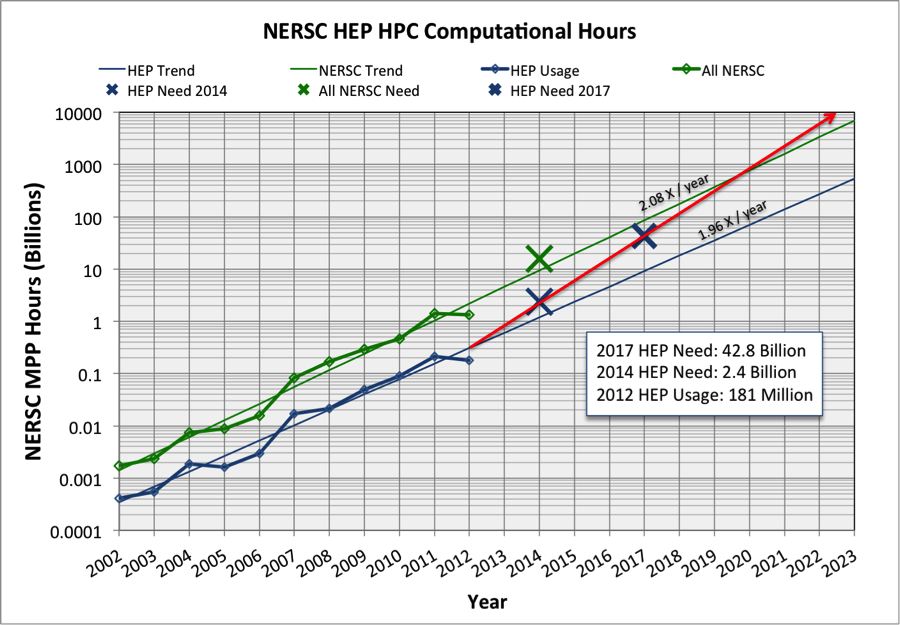
\includegraphics[width=\textwidth]{CpF-I2/images/2013-NERSC-Usage-HEP.png}
\caption{Historical normalized computing hours used at NERSC (green line) and just for HEP projects (blue line). Results from NERSC requirements reviews with HEP scientists and DOE program managers (large blue crosses) show a need for computing greater than what will be supplied by extrapolating the trend.}
\label{fig:NERSC-Computational-Hours}
\end{figure}


One effort, Perturbative QCD,  that has largely relied on HTC computing to date has already started using HPC centers and expects to 
expand those efforts to be able to complete the calculation of important background and signal reactions at the
LHC.  
They have determined that it would be beneficial to make the national DOE HPC
facilities 
generally accessible to particle theorists and
experimentalists in order to enable the use of existing
calculational tools for experimental studies involving extensive
multiple runs without depending on the computer power and manpower
available to the code authors. Access to these facilities will also
allow prototyping the next generation of parallel computer programs
for QCD phenomenology and precision calculations.

 
\section{Future Availability of Resources}


The needed computing resources for Energy Frontier experiments are currently set by the needs of the CMS and ATLAS experiments.  Both of these experiments have had several years of running experience and have developed the tools to predict future resource needs as a function of experimental parameters such as the trigger rate, pileup distribution, event size, number of reprocessing and analysis passes per year and so forth.  These models have been shown to be reasonably predictive~\cite{bib:CHEPresources}.

It currently appears that the needs will be met for the foreseeable ($\sim$10 year) future as long as several conditions are satisfied.  So far, the funding for the WLCG has been roughly constant, allowing resource growth to continue with Moore's Law.  Experiments have been able to adjust their computing models to adapt to the available growth in resources along with the growth in data sets.  While Moore's Law does not seem to hold as well as it used to, resources should still grow over time, although not as quickly as before.  Near-constant WLCG funding will be necessary for the experiments to keep up with growing datasets and event complexity.  

Meanwhile, computing architectures are changing, and the experiments' software bases must evolve to keep up with them.  Adapting the software to take advantage of many-core and multicore processor architectures is also critical for LHC experiments to meet their computing needs.  The experiments will also need to find greater efficiencies in resource usage, for both processing and disk resources.  Currently both ATLAS and CMS distribute many datasets to their computing sites that are subsequently rarely or never used; this is then a waste of storage.  The experiments will also need to proactively pursue and take advantage of a variety of resources beyond the WLCG.  These include opportunistic resources that might be available at universities, laboratories and NSF and DOE computing centers, and paid resources that might be available through commercial clouds.  Fortunately, both CMS and ATLAS are actively pursuing many of these measures, which are an important part of the development plans underway during the current LHC shutdown.

Intensity Frontier experiments have relatively modest computing needs, at least in comparison to those of the Energy Frontier experiments.  Any single such experiment is expected to produce ``only'' a petabyte of data over its entire lifetime, compared to CMS or ATLAS which will produce several petabytes per year.  Thus it should not be difficult to provide the needed scale of computing resources for these experiments as long as sufficient funds are available.  These experiments too will be able to help themselves by actively pursuing opportunistic resources and operational efficiencies as the Energy Frontier experiments are.

Cosmic Frontier experiments have well-defined storage needs, and these become competitive with those of CMS and ATLAS in future years.  The Dark Energy Survey should produce ``only'' a petabyte of data by 2016 (well within current capabilities), but LSST could produce 100 PB by 2030.  The Square Kilometer Array could produce as much as 1500 PB/year when it is operational in the 2020's.  In addition, these experiments could have very different access and processing patterns than those of the accelerator-based experiments.  

The large increase in survey data means that statistical noise will no longer determine the accuracy to which cosmological parameters are 
measured. The control and correction of systematic uncertainties will determine the scientific impact of any cosmological survey. 
Achieving the goals of current and planned experiments will, therefore, require the processing and analysis of experimental data streams, 
the development of techniques and algorithms for identifying cosmological signatures and for mitigating systematic uncertainties, 
 and detailed cosmological simulations for use in interpreting systematic uncertainties within these data. 

There are three primary computational tasks associated with sky surveys: image generation, image processing, and cosmological simulation. The first 
is primarily an HTC task, the second is alredy running in HPC mode using up to thousands of processors, and the third uses cutting-edge HPC applications.  The computing requirements for image simulation and image processing will increase greatly over the next five years and, while substantial
on the order of 100 million hour, are expected to be accomodated at DOE and NSF centers. The HPC hours needed for cosmological simulations are extreme, however, reaching 10s of billions of hours by 2017 (reference NERSC report). The current outlook
makes it unlikely that HPC centers have adequate capacity to meeting these needs for cosmological
simulations on this time scale. 
 
Likewise, researchers performing Lattice QCD theory calculations 
-- which are essential for interpretation of many experiments done in high-energy and nuclear physics -- 
face an expected deficit in computing cycles. In in a recent report (cite NERSC report) 
LQCD researchers estimate needing 10s of billions of  hours in 2017, much more than will be available 
for LQCD if historical trends hold.

HPC needs for accelerator research and design are growing, too, but are expected to be accommodated by planned HPC center capacity and capability increases (cite NERSC report). 

